%%%%%%%%%%%%%%%%%%%%%%%%%%%%%%%%%%%%%%%%%%%%%%%%%%%%%%%%%%%%%
%
% Section: Functions and Mathematical Models
%
%%%%%%%%%%%%%%%%%%%%%%%%%%%%%%%%%%%%%%%%%%%%%%%%%%%%%%%%%%%%

\section{Functions and Mathematical Models}

A function does not have to be useful. If a rule gives one and only one output for each input, it’s a function. A useful application is not required. $f(x)=x^2$ is a perfectly good function because whenever you square a number you get one and only one result. This is true regardless of whether or not we have any useful reason for squaring numbers.\\

We make no apologies for sometimes doing mathematics with no obvious application to develop and practice ideas, skills and techniques (just as a football coach makes no apologies for running drills and doing exercises that are not themselves actually part of any football game). But we also do want to keep in mind that most people study mathematics because it is useful for something else they want or need to do!

%%%%%%%%%%%%%%%%%%%%%%%%%%%%%%%%%%%%%%%%%%%%%%%%%%%%%%%%%%%%%
%
% Subsection: Functions and Mathematical Models: Functions as Models
%
%%%%%%%%%%%%%%%%%%%%%%%%%%%%%%%%%%%%%%%%%%%%%%%%%%%%%%%%%%%%

\subsection{Functions as Mathematical Models}

When we use mathematical tools to describe something about the world, we say we are using a \textbf{mathematical model}\index{Mathematical Model}. Functions are a natural tool for mathematical modeling.\\

Suppose, for example, that you are pumping water out to drain a swimming pool. The pool started out full, with a volume of 7200 gallons of water, and the pump is pulling out a steady 20 gallons per minute. There is a relationship here between the time that has passed since the pump started and the remaining volume of the pool, and we would like to be able to set up a mathematical model for this relationship using a function.\\

To do this we first need to decide which quantity should be the input and which should be the output. The more natural way to do this would be to treat volume as a function of time, since the volume is changing as the time changes. Also, at any given time the pool can only have one volume (i.e. it is impossible for the pool to have two different volumes at the same time!), so we know setting things up this way will meet the requirements of a function. So our mathematical model would be based on a function like this:

\begin{equation*}
	time \rightarrow \boxed{f} \rightarrow volume
\end{equation*}

Could we do it the other way around? Sometimes we can set up a model with inputs and outputs switched, and which way we do it depends on which approach we find more convenient or useful.  Sometimes we can’t because the model only works as a function one way, In this example, we would run into some trouble if we tried to set things up with time as a function of volume, like this:

\begin{equation*}
	volume \rightarrow \boxed{f} \rightarrow time
\end{equation*}

The problem is that the pool actually will have the same volume at two different times. When will the pool be empty? Well, it will be empty at the moment the pump finishes draining it. But it will also be empty a minute after that! So, if you input a volume of zero gallons, you could get more than one output of time when the volume is zero gallons. When is the pool full? Well, it’s full when the pump first starts to run, but it also was full a minute before that. So we run into the same
problem there as well.\\

We could work around this if we had to, for example by adding that we only want to know the time while the pump is running that the pool is at the input volume. So, it actually might be possible to set up a function model with time as a function of volume, but this makes things much more complicated. So our original plan of setting up a model with volume as a function of time seems the best bet.

\exam{\label{FunctionsasModelsExample1} To set up a function to mathematically model each of the following, which quantity is the more natural choice for input and which is the more natural choice for output? Explain your reasoning, and state your answer in the form \quotes{ should be a function of }.
	\begin{enumerate}[label=(\alph*)]
		\item You are shooting a model rocket upward, and measuring its height over the course of its flight.
		\item Your monthly electric bill is based on the amount of electricity you use.
	\end{enumerate} 
}

\indenttext{
	\begin{enumerate}[label=(\alph*)]
		\item The two quantities are time since launch and height. It is probably more natural to think of height as a function of time (i.e. you input time and the model tells you the rocket’s height). This also works as a function, because at each time (input) the rocket can only be at one height (output) - the rocket can’t be in two different places at once.\\
		\newline
		On the other hand, if we try to use height as the input, we run into trouble, since the rocket will be at the same height at more than one time. If you ask, say, when the rocket will be $15$ feet above the ground, there can be two different answers: when it reaches that height on the way up and also on the way down. So we cannot have a function that uses height as the input and gives time as the output.\\
		\newline
		So, we must set this up with time as the input and height as the output. In other words, height should be a function of time.
		\item This could probably be set up either way. If you use a certain amount of electricity, the utility company will send you one and only one bill for that use - they never send you two different bills and let you pick which you want to pay. So if we input electric use, we get one and only one bill amount.\\
		\newline
		On the other hand, if we know your bill for the month, there probably is only one amount of electric use that would give you that bill, since if you use less it would probably be lower and if you use more it will probably be higher. So, we could probably set this up with bill as input and electric use as output.\\
		\newline
		It seems more natural though, to set up the function like this:
		\begin{equation*}
			electricity \text{ } use \rightarrow \boxed{f} \rightarrow bill
		\end{equation*}
		because this more closely reflects the way you are most likely to look at this relationship. In reality, you use a certain amount of electricity and then the utility uses that information to determine your bill. The other way around - taking the amount of your bill and using it to determine how much electricity you use - could make sense if you were thinking about managing your electric use to fit a budget, but is a less natural way of looking at things.\\
		\newline
		So, we would probably set this model up with the bill amount being a function of electric use.
\end{enumerate} 
}

Once we have determined our input and output, we next need to find a formula or other rule that fits the scenario we are trying to model. Finding formulas to suit mathematical models will be a major topic of the rest of this course and book, so we won’t get too deeply into that quite yet. You are not expected to come up with formulas on your own yet. For the swimming pool problem, we will note here that the pool starts with $7200$ gallons and since it is pumping at a rate of $20$ gallons per minute, after $t$ minutes $20t$ gallons will have been pumped out. Putting that together, it turns out that the volume of water in the pool as a function of time since the pump was turned on can be mathematically modeled with the function

\begin{equation*}
	f(t)=7200-20t
\end{equation*}

where $f(t)$ is the volume of water after $t$ minutes of pumping and $t$ is the minutes the pump has been running.\\

While we are not going to spend much time trying to find formulas yet, we are interested in how a formula can be used to get information about the relationship we are mathematically modeling.  Suppose, for example, we want to know how much water will be left in the pool after one hour. We can use this model to answer this question. Time is the input for this function, so we can input into it a time of one hour. Since $t$ is the time in minutes, this means we need to input $t=60$ (since an hour is $60$ minutes). So, doing this we get:

\begin{equation*}
	f(60)=7200-20(60)=6000
\end{equation*}

The output we get from the model is a value of $6000$. Since the output is the gallons of water left in the pool, we can conclude that \quotes{after the pump has been running for an hour, the volume of water in the pool is $6000$ gallons.}  Or, phrased a little more naturally, \quotes{there are $6000$ gallons of water left in the pool after the pump has been running for one hour.}

\exam{\label{FunctionsasModelsExample2} Suppose that your electric bill in dollars as a function of your monthly electric usage in kilowatt hours is given by $b(x)=7.95+0.1x$.   Determine your electric bill if you use $800$ kilowatt hours.}

\indenttext{Since usage is the input, we need to input $x=800$ into our function model. So:
	\begin{equation*}
		b(800)=7.95+.1(800)=87.95
	\end{equation*}
	Interpreting this we would say something like this: \quotes{if you use $800$ kilowatt hours, your bill will be $\$87.95$.}
}

\exam{\label{FunctionsasModelsExample3} Suppose that the height of a toy rocket in feet $t$ seconds after it is launched is given by the function $h(t)=-16t^2+96t$.  What is the rocket’s height $3$ seconds after launch?}

\indenttext{Since time is the input, we know we need to input $t=3$ into our function model:
	\begin{equation*}
		h(3)=-16(3)^2+96(3)=144
	\end{equation*}
	Of course, \quotes{$h(3)=144$} is not a very good answer to the question asked; if you asked someone what the rocket’s height would be and they answered \quotes{$h(3)=144$} you’d probably find that a weird way of answering your question!  Interpreting the function to answer the question in a reasonable way, we would say something like this: \quotes{the height of the rocket $3$ seconds after launch will be $144$ feet.}
}
\bigskip

In both of the examples, we knew the input and used our model to get the output. That is usually the way we want our mathematical models to work. It only makes sense that we would want functions set up to take as input the information we are most likely to start with, and give as output the information we are seeking. However, it doesn’t always work that way!\\

Returning to our pool example, suppose we want to know how long it will take to completely pump the water out of the pool? In other words, we want to know when the volume of the pool reaches zero. So we know the volume (the function’s output) and want to know the time (the function’s input). Even though this is kind of backwards from the way we set up our function, we can still figure this out. Here, we know the volume (output) needs to be zero, so we plug in $f(t)=0$ for the
output:

\begin{align*}
	f(t)&=7200-20t\\
	0&=7200-20t
\end{align*}

and then solve the equation we get using algebra:

\begin{align*}
	20t&=7200\\
	t&=360
\end{align*}

So, the time when we reach a volume of $f(t)=0$ gallons is $t=360$ minutes. So we might say \quotes{the pool will be empty after $360$ minutes of pumping.} Even better, since the amount of time is longer than we usually measure in minutes, we might convert this to hours. Since there are 60 minutes per hour, there are 360 = 6 hours here, so an even better answer might be \quotes{the pool will be emptied after 6 hours of pumping}.

\exam{\label{FunctionsasModelsExample4} Suppose that your electric bill in dollars as a function of your monthly electric usage in kilowatt hours is given by $b(x)=7.95+0.1x$.  If your electric bill last month was $\$92.55$, how 	much electricity did you use?}

\indenttext{
	Since we know the bill (output) is $\$92.55$, we plug $b(x)=92.55$ into our model and solve to find $x$:
	\begin{align*}
		b(x)&=7.95+0.1x\\
		92.55&=7.95+0.1x\\
		84.6 &= 0.1x\\
		x &= 846
	\end{align*}
	So, in answer to the original question: \quotes{if your bill was $\$92.55$ you must have used $846$ kilowatt hours of electricity.}
}
\bigskip

Since function formulas are set up to give an output when you plug in an input, when we do the opposite we always end up with an equation to solve. Sometimes, as in the preceding example, we can do this effectively with algebra. Other times, as in the following example, we may need to call on graphical solution.

\exam{\label{FunctionsasModelsExample5} Suppose that the height of a toy rocket in feet $t$ seconds after it is launched is given by the function $h(t)=-16t^2+96t$. When is the rocket $100$ feet above the ground (rounded to two decimal places if necessary)?}

\indenttext{We know the height (output) we want, so we plug in $h(t)=100$ to get the equation:
	\begin{equation*}
		100=-16t^2+96t
	\end{equation*}
	Now, if we use the standard window, we don’t wind up with a very helpful view of this graph. What window should be use? We know something about the equation we are trying to solve here; we know that the input represents time since launch, and the output represents height of the toy rocket. This gives us good hints about how to adjust out window.\\
	\newline
	For the input values, we are looking at values that might make sense for the time when the rocket is at $100$ feet. Now, we don’t know when this actually happens, of course, but we do have some sense of what is reasonable. Certainly the rocket can’t possibly have been at $100$ feet before it was launched, so it makes no sense to look at input values less than zero. How long might it take for the rocket to hit $100$ feet? We can make a reasonable guess (knowing that if the graph doesn’t look reasonable based on this guess we can always change it.) Let’s say we guess 3 seconds.\\
	\newline
	For the output window, we know we are looking for a height of $100$ feet, which tells us we certainly want to have a window that includes $100$. Since we are talking about shooting a rocket off the ground, it seems reasonable to look at heights from $0$ to a bit above $100$, say $125$.\\
	\newline
	So, we set our window to be:
	\begin{figure}[H]
		\centering
		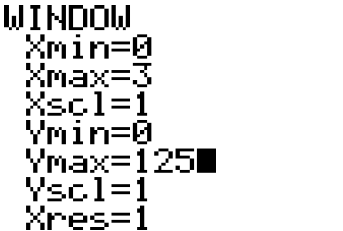
\includegraphics[scale=1.0]{Sections/FunctionsasModelsImages/Figure01.png}
		\caption{Window Settings}
	\end{figure}
	Giving the resulting graph:
	\begin{figure}[H]
		\centering
		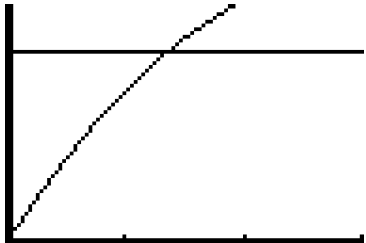
\includegraphics[scale=0.8]{Sections/FunctionsasModelsImages/Figure02.png}
		\caption{Graph for $Y_1=-16x^2+96x$ and $Y_2=100$}
	\end{figure}
	Which, using graphical solution, gives us the solution $t=1.34$: the rocket reaches $100$ feet above the ground $1.34$ seconds after launch.\\
	
	Now, we are not done! This model represents the flight of a toy rocket. We’ve found then it hits $100$ feet on the way up, but common sense tells us that it will also hit $100$ on the way down, which we do not see in our graph. It must be that the rocket falls to $100$ feet some time after $3$ seconds as well, so we need to extend our input (X) maximum to see this. We can also tell from looking at our graph that the rocket actually goes higher than $125$ feet, so we may want to increase the output (Y) maximum as well – though this is not really necessary to solve the equation, doing so may make us feel better about the graph we’re using.\\
	
	So, adjusting out window out a ways, such as:
	
	\begin{figure}[H]
		\centering
		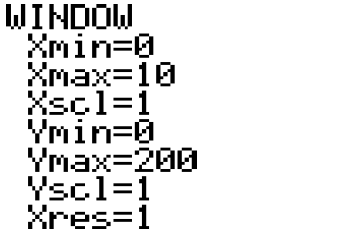
\includegraphics[scale=1.0]{Sections/FunctionsasModelsImages/Figure03.png}
		\caption{Adjusting Window Settings}
	\end{figure}
	
	We get a new view of the graph:
	
	\begin{figure}[H]
		\centering
		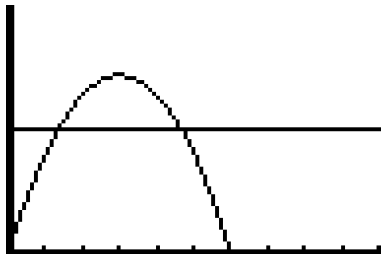
\includegraphics[scale=0.8]{Sections/FunctionsasModelsImages/Figure04.png}
		\caption{Graph for $Y_1=-16x^2+96x$ and $Y_2=100$}
	\end{figure}
	
	And solving for that second intersection we get $t=4.66$\\
	
	So we conclude that the rocket is $100$ feet above the ground $1.34$ seconds after launch on the way up, and $4.66$ seconds after launch on the way down.
}

\bigskip

Having a mathematical model actually makes graphical solution easier! In this example, it both helped us figure out an appropriate window, and also tipped us off that the one intersection we say in our first window wasn’t the only solution.\\

Don’t worry about picking precisely the right window with these types of problems; there is no absolutely right window. Example \ref{FunctionsasModelsExample5} could have been done just as well with some different window choices. How did we know to try a max of 3 seconds on the first try, as opposed to 5 seconds or 2 seconds? We didn’t! It was just a reasonable thing to try as a first attempt. Your goal should be to make a reasonable, educated guess, and if that guess turns out not to fit what the facts should be, to adjust it. But you are not guessing blindly when you have a mathematical model; the meaning of the model can and should give you hints.

%%%%%%%%%%%%%%%%%%%%%%%%%%%%%%%%%%%%%%%%%%%%%%%%%%%%%%%%%%%%%
%
% Subsection: Functions and Mathematical Models: Interpreting Function Notation
%
%%%%%%%%%%%%%%%%%%%%%%%%%%%%%%%%%%%%%%%%%%%%%%%%%%%%%%%%%%%%

\subsection{Interpreting Function Notation}

If you are given information about a function used in a mathematical model, you do not necessarily need to know the formula or rule for that function in order to interpret that information. It is possible, and desirable, to translate between function notation and interpretations, regardless of whether we have a formula.\\

For example, suppose you are told that the function $f(t)$ gives the volume of water (in gallons) in a pool as a function of time in minutes since we began pumping water out of the pool, and suppose you are also told $f(10)=7000$.  You do not need the formula to interpret what that means!\\

You know that volume of water is a function of time, and so that means time is the input and water is the output (because it is always \quotes{output is a function of input}.)\\

You also know that function notation is always \quotes{$f(input)=output$}. So:

\begin{equation*}
	f\left(\underbrace{10}_{input} \right)=\underbrace{7000}_{output}
\end{equation*}

So $10$ in the input and input is time, so that must mean \quotes{10 minutes}. Likewise, $7000$ is the output and output is volume of water, so that must mean \quotes{7000 gallons}. Putting these facts together, we can interpret that as saying \quotes{when time is 10 minutes, the volume of water is 7000 gallons}. Since that’s kind of an awkward way of saying it, though, we might want to rephrase that a little more naturally as something like:

\begin{center}
	\quotes{after 10 minutes of pumping, 7000 gallons of water is left in the pool}.
\end{center}

We can go the other way too. Suppose you know that there are 4800 gallons of water left after 2 hours (120 minutes). Time is the input, so the input is 120. Volume is the output, so the output is 4800 gallons. So, following the format $f(input)=output$ we can write this in function notation as:

\begin{equation*}
	f(120)=4800.
\end{equation*}

\exam{\label{FunctionsasModelsExample6} The amount of yeast (in teaspoons) needed for bread dough is a function of the amount of dough being made (in pounds). Interpret $f(4)=6$}

\indenttext{\quotes{Yeast is a function of dough} here, so yeast is the output and dough is the input. Also, \quotes{$f(4) = 6$} so $6$ is the output value and $4$ is the input value.\\

Putting this together means we have $4$ pounds of dough and $6$ teaspoons of yeast. Phrasing this in a reasonable way gives an answer something like \quotes{you need 6 teaspoons of yeast to make 4 pounds of dough}.
}

\exam{\label{FunctionsasModelsExample7} A realtor’s commission is a function of the selling price of the real estate sold.  Suppose the realtor receives $\$4,800$ for selling a property for $\$160,000$. Express this in function notation.  Assume the function’s name is $f(x)$.
}

\indenttext{\quotes{Commission is a function of selling price} so commission is the output and selling price is the input.\\

	Also,$f(input)=output$, so following this format we would write $f(160,000) = 4,800$.
}

%%%%%%%%%%%%%%%%%%%%%%%%%%%%%%%%%%%%%%%%%%%%%%%%%%%%%%%%%%%%%
%
% Subsection: Functions and Mathematical Models: Relevant Domain and Range
%
%%%%%%%%%%%%%%%%%%%%%%%%%%%%%%%%%%%%%%%%%%%%%%%%%%%%%%%%%%%%

\subsection{Relevant Domain and Range}

\index{Function!Relevant Domain} \index{Function!Relevant Range}
We have previously defined domain to be the set of all the inputs for a function. Most of the functions we are interested in for this course involve numerical values, and as we’ve seen the domain for these functions will usually be all real numbers (except where we need to restrict the domain to avoid dividing by zero or taking the square root of a negative.)\\

So, for example, the domain of the function

\begin{equation*}
	f(t)=7200-20t
\end{equation*}

would be all real numbers, since we can plug in any real number for $t$, evaluate the result, and get one and only one output. So, for examples, $t=0$, $t=120$, $t=5,000,000,000$, and $t=-317,432$ would all be in the domain of this function, since these are all real numbers which can be substituted into the formula and give one and only one output as a result.\\

When we are looking at functions as purely abstract things, our only concern is whether or not we get a single output for a given input. When we are using functions as mathematical models, though, that’s not all that we care about. The function mentioned above you no doubt will recognize as the pool-draining function we’ve been using in this chapter. In that model, $t$ is not just the value you input – it actually represents something. Plugging in $t=0$ means that we are looking at what happens when no time has passed, when the pump is just first turned on. Plugging in $t=120$ means that we are looking at what happens after $120$ minutes.\\

And so plugging in $t=5,000,000,000$ means that we are looking at what happens after the pump has been running for five billion minutes. This poses no problem with the formula – we can plug that in and evaluate the result just fine – but does that actually make any sense? Does $t=-317,432$ really make any sense? Would we really plug this in to use our model to find how much water was in the pool $317,432$ minutes before the pump is turned on? Again, there’s no problem
doing the calculation – but do we really expect that calculation to tell us anything worthwhile?\\

In the context of pumping water out of the pool, it really only makes sense to look at times between when the pump is first switched on and when the pool is completely drained. The pump is switched on at time $t=0$ and, we calculated earlier in this section, the pool is fully drained at time $t=360$.\\

So realistically speaking, the domain for the function in this mathematical model would be all real numbers between $0$ and $360$ inclusive, which we would write as

\begin{equation*}
	\{t|0 \leq t \leq 360\} \text{    OR    } [0,360]
\end{equation*}

So, we really have two different \quotes{domains} for this function. The domain in the abstract sense is all real numbers, because any real number can be input into the function and give one and only one output. When we say \quotes{domain} in mathematics, this is what we are talking about.\\

The domain in the sense of things that we actually would meaningfully input into this model, though, is this more limited one. We call this the relevant domain. So, for the function $f(t)=7200-20t$ the domain is all real numbers. For this function within the mathematical model we are discussing, the relevant domain is all real numbers from $0$ to $360$ inclusive.\\

We do something similar with range. The range is the set of all outputs for the function. We didn’t spend much time finding function’s ranges, because that really requires more advanced algebra tools. But the relevant range for a given mathematical model is often easier to determine. In our swimming pool example, the output represents the gallons of water in the pool. We know that the pool starts with $7200$ gallons and we are draining it, so we would expect that any volume between $0$ and $7200$ gallons would be a reasonable output to get. So the relevant range would be

\begin{equation*}
	\{f(t)|0 \leq f(t) \leq 7200\} \text{    OR    } [0,7200]
\end{equation*}

We won’t worry about what the range of this function is in the abstract sense here, other than to note that it would include plenty of values that would make no sense as the volume of water in the pool. For example, if you solve the equation $-2,000,000=7200-20t$ you get an answer, so $-2,000,000$ would be in the range of this function, since solving this equation shows that it is possible to get $-2,000,000$ as an output. But it certainly it makes no sense to ask when there are
negative two million gallons of water in the pool.\\

In the pool-draining example it is pretty clear what the relevant domain and relevant range must be.  The action starts when the pump is turned on and ends when the pool is drained, and that determines the relevant domain and relevant range. This is not always so clear cut; sometimes the line between what would be reasonable and what wouldn’t is fuzzy, and we have to accept some ambiguity. The following example will illustrate:

\exam{\label{FunctionsasModelsExample8} The speed limit on the Pennsylvania Turnpike is $65$ mph. The fine for speeding as a function of how fast you were going is given by the function $f(s)=75+5(s-65)$
	\begin{enumerate}[label=(\alph*)]
		\item Regarded as an abstract function, what is the domain of $f(s)$?
		\item What would be a reasonable choice for the relevant domain and relevant range for this function as a mathematical model?
\end{enumerate} 
}

\indenttext{
	\begin{enumerate}[label=(\alph*)]
		\item Any real number could be input into this formula to get one and only one output. So the domain is all real numbers.
		\item Since fine is a function of speed, the input is speed and the output is the fine. So, the relevant domain would consist of all possible speeds you could be going when caught speeding.  Since the speed limit is $65$ mph, you could not be caught speeding unless your speed was at least 	$65$ mph. Realistically, though, you almost certainly wouldn’t get a ticket for doing, say $66$ or $67$ mph. But it’s not really possible to say exactly where the cut off is. It might be reasonable to use a lower limit of $68$ or $70$ mph, or to just keep it simple and use a lower limit of $65$ mph anyway, since even though you’re not likely to be stopped for speeding going slightly over 65, you could be.  We’ll use a lower limit of 65.\\

		At the upper end, clearly there are some speeds that you could not possibly reach. I think it’s pretty clear for example that no one will get a ticket for going $20,000$ mph! Even $200$ mph is not a realistic possibility. But is $90$ mph possible?  Well, not in my car, but yes it is possible that a car could be going that fast. $100$ mph? That’s pushing it, but is it possible? Sure. $110$ mph?  Unlikely, but not out of the question. What is the absolute upper limit? It’s really not possible to say. Clearly, the relevant domain has some upper limit, and it’s probably somewhere in the low $100$’s, but it’s impossible to say exactly where it is. We’ll use an upper limit of $125$ mph.\\

		Putting this all together, we get a relevant domain of $\{s|65 < s \leq 125\}$ or $(65,125]$. This is a good answer – but it is not the only possible good answer. We did not include 65 since going exactly 65 would not be speeding, but it would still not be entirely unreasonable to include it and give the relevant domain as $\{s|65 \leq s \leq 125\}$ or $[65,125]$.  Also, as we discussed, a different lower or upper limit could be used. It would also be reasonable to give an answer of $\{s|67 \leq s \leq 120\}$ or $[67,120]$ for example. As long as the lower and upper bounds for the relevant domain make sense as lower and upper bounds for how fast you could be going when stopped for speeding, you’ve got a reasonable relevant domain.\\
		
		The relevant range has the same issues – there is not a single correct answer for this. But, the fine does depend on speed, so our relevant range should be consistent with the speeds we included in our relevant domain. The fine goes up with higher speeds, so the lowest fine would be the fine based on the lowest speed, and the highest fine would be based on the highest speed.  Since we used $s=65$ as the lower limit for speeds, we should use $\$75$ as the lower limit for fines, since $f(65)=75+5(65-65)=75$ would be the fine for that speed.  For the upper limit of $s=125$, the fine would be $f(125)=75+5(125-65)=375$ dollars. So our relevant range would be $\{f(s)|75 \leq s \leq 375\}$ or $[75,375]$. (If we used a different relevant domain, we would set up the relevant range based on that.)
	\end{enumerate} 
}

Graphing can also be a useful tool in determining relevant domains and ranges.

\exam{\label{FunctionsasModelsExample9}A toy rocket is launched from the ground. Suppose that the height of a toy rocket in feet $t$ seconds after it is launched is given by the function $h(t)=-16t^2+96t$.  What would be reasonable choices for the relevant domain and relevant range of this function?
}

\indenttext{Time is the input and height is the output. The relevant domain would be all reasonable times to use in this model, which is clearly the time between when the rocket is launched and when it returns to the ground. When the rocket is launched, $t=0$ so that is pretty clearly the lower limit for the relevant domain. The upper limit would be when the rocket returns to the ground. To find this we would need to plug in $h(t)=0$ into the function, and then solve
	\begin{equation*}
		-16t^2+96t=0
	\end{equation*}
	Solving this equation with algebra is beyond our present abilities, but we can solve this graphically.  Doing so, we find that the rocket returns to the ground at time $t=6$ seconds after launch.\\

	So, our relevant domain is $\{t|0 \leq t \leq 6\}$ or $[0,6]$. There is no ambiguity about this – this is really the only reasonable relevant domain to use.\\

	Since height is the output, the relevant range would be based on the heights the rocket actually reaches. In this case we cannot just base this on the upper and lower limits of our domain because the height is not always increasing – the rocket hits its maximum height during its journey.\\

	We can find this maximum using the graphing calculator’s built-in programs, following these steps:
	\index{Calculator:Maximum}
	\begin{itemize}
		\item Create the graph in an appropriate window, in which the maximum occurs.
		\item Hit \quotes{2nd} \quotes{TRACE} (i.e. \quotes{CALC}) $\rightarrow$ \quotes{4: maximum} --> \quotes{ENTER}
		\item For \quotes{Left Bound?} choose any X-value to the left of the maximum and hit \quotes{ENTER}
		\item For \quotes{Right Bound?} choose any X-value to the right of the maximum and hit \quotes{ENTER}
		\item For \quotes{Guess?} move the blob reasonably close to the maximum if there is more than one place where the graph reaches a peak, otherwise just hit \quotes{ENTER}
		\item The calculator will find the maximum.
	\end{itemize}
	Since the maximum height is $144$ feet, the relevant range is $\{h(t)|0\leq h(t) \leq 144 \}$, or $[0,144]$.
}

%%%%%%%%%%%%%%%%%%%%%%%%%%%%%%%%%%%%%%%%%%%%%%%%%%%%%%%%%%%%
%
% Subsection: Functions and Models: Exercises
%
%%%%%%%%%%%%%%%%%%%%%%%%%%%%%%%%%%%%%%%%%%%%%%%%%%%%%%%%%%%%

\clearpage

\subsection{Exercises}

\subsubsection*{Functions as Mathematical Models}

\textbf{1-16:} To set up a function to mathematically model each of the following, which quantity is the more natural choice for input and which is the more natural choice for output? Explain your reasoning, and state your answer in the form \quotes{\underline{\phantom{blank}} should be a function of \underline{\phantom{blank}}}.

\bigskip
\ex{The cost to mail a package is calculated based on its weight.}
\sol{Cost is a function of weight.  Weight determines cost; your start with the package weight and from it you determine cost.}

\bigskip
\ex{The sales tax charged for a purchase is calculated based on its cost.}

\bigskip
\ex{The interest rate charged for a loan is based on the borrower’s credit score.}
\sol{Interest rate is a function of credit score.  Credit score determines the rate charged.}

\bigskip
\ex{A contractor bases his charge for paving a parking lot on the lot’s area.}

\bigskip
\ex{The air pressure in a tank depends on the mass of the air contained in the tank.}
\sol{Air pressure is a function of mass.  \quotes{Depends on} tells us that the air pressure is a function of the mass.}

\bigskip
\ex{The amount of air contained in a tank depends on the pressure inside the tank.}

\bigskip
\ex{A scientist is studying the radiation level measured in the water near a nuclear power plant over time after a leak.}
\sol{Radiation level is a function of time.  You are more likely to give a time and determine what the radiation level was then than you are to go the opposite 
way.}

\bigskip
\ex{An online music site uses the number of songs you download to determine your monthly membership charge.}

\bigskip
\ex{An insurance company uses an employer’s total unemployment claims from the prior three years to determine the company’s unemployment insurance premium.}
\sol{Premium is a function of claims.  The claims are used to determine the premium.}

\bigskip
\ex{A publisher is recording the sales of a book over time since it was first published.}

\bigskip
\ex{The Richter scale rating of an earthquake is calculated from the amount of energy released in the quake.}
\sol{Richter scale is a function of energy.  The problem states that Richter scale is calculated from energy.}

\bigskip
\ex{The category level of a hurricane is determined by its maximum wind speed.}

\bigskip
\ex{An entomologist believes that the pitch at which crickets chirp changes as the air temperature changes.}
\sol{Pitch is a function of temperature.  You might be able to do this either way, but it is more natural to think of the function this way since temperature would 
cause the pitch to change and not vice versa unless you have powerful weather-controlling crickets.}

\bigskip
\ex{The remaining run time for an iPod changes as the remaining charge on the battery changes.}

\bigskip
\ex{There is a relationship between the size of a file and the time that your download manager will estimate it will take to download.}
\sol{Download time is a function of the file size.  File size determines the download time.}

\bigskip
\ex{There is a relationship between your weight and the age to which a life insurance company will predict that you will live.}

\bigskip
\noindent \textbf{17-30:} Each of the following questions defines a function, and asks you to determine something based on that function. State your answers in ordinary English (i.e. without using function notation or mathematical jargon.) Where necessary round your answers to two decimal places.

\bigskip
\ex{A club is planning a field trip to Washington D.C. The total cost of the trip is a function of the number of members who will be going, and is given by the formula $c(x)=1850+475x$. What will the total cost be if $30$ members go?}
\sol{$\$16,100$}

\bigskip
\ex{The amount of music (in hours) that you want to be able to store on a digital music player determines the amount of memory capacity (in megabytes) it must have. The needed capacity is given by the formula $m(x)=10x+120$. How much capacity would be needed to be able to store 750 hours of music?}

\bigskip
\ex{The amount of music (in hours) that can be stored on an digital music player is a function of the size of its memory capacity (in megabytes), and is given by the formula $t(x)=\frac{x-120}{10}$. How much music can be stored on a player with a $6000$ megabyte capacity?}								
\sol{588 hours}

\bigskip
\ex{A club is planning a field trip to Washington D.C. The cost per person for the trip is a function of the number of members who will be going. This function is given by the formula $f(x)=\frac{180+475x}{x}$. What will the cost per person be if $25$ members go?}

\bigskip
\ex{The time it takes (in seconds) for a baseball thrown upward to reach its maximum height above the ground is a function of the initial upward velocity with which it is thrown (in feet per second). This function is given by the formula $t(v)=\frac{v}{32}$. How long will it take a ball thrown upward with an initial velocity of $80$ feet per second to reach its maximum height?}
\sol{2.5 seconds}

\bigskip
\ex{The time it takes (in seconds) for a baseball thrown upward to reach its maximum height above the ground is a function of the initial upward velocity with which it is thrown (in meters per second). This function is given by the formula $t(v)=\frac{5v}{49}$. How long will it take a ball thrown upward with an initial velocity of $32.5$ meters per second to reach its maximum height?}

\bigskip
\ex{Your total state income tax is a function of your taxable income, and can be calculated from the formula $f(x)=1000+0.08(x-30,000)$ when your taxable income exceeds $\$30,000$.  Determine your income tax if your taxable income is $\$42,000$.}
\sol{$\$1,960$}

\bigskip
\ex{A club is planning a field trip to Washington D.C. The total cost of the trip is a function of the number of members who will be going, and is given by the formula $c(x)=1850+475x$. If the club has budgeted a total cost of $\$18,950$, how many people are they expecting will go?}

\bigskip
\ex{The amount of music (in hours) that you want to be able to store on a digital music player determines the amount of memory capacity (in megabytes) it must have. The needed capacity is given by the formula $m(x)=10x+120$. How much music could be stored on a player with a $6000$ megabyte capacity?}
\sol{588 hours}

\bigskip
\ex{The amount of music (in hours) that can be stored on an digital music player is a function of the size of its memory capacity (in megabytes), and is given by the formula $t(x)=\frac{x-120}{10}$. How much capacity would be needed to store $750$ hours of music?}

\bigskip
\ex{The time it takes (in seconds) for a baseball thrown upward to reach its maximum height above the ground is a function of the initial upward velocity with which it is thrown (in feet per	second). This function is given by the formula $t(v)=\frac{v}{32}$. If the ball reaches its maximum height $2.8$ seconds after being thrown, what was its initial upward velocity?}
\sol{89.6 feet per second}

\bigskip
\ex{The time it takes (in seconds) for a baseball thrown upward to reach its maximum height above the ground is a function of the initial upward velocity with which it is thrown (in meters per second). This function is given by the formula $t(v)=\frac{5v}{49}$. If the ball reaches its maximum height $3.5$ seconds after being thrown, what was its initial upward velocity?}

\bigskip
\ex{A contractor is building a square pool with a $3$ foot deck surrounding it. The total area taken up by the pool and its deck (in square feet) is a function of the length of the pool’s side (in feet), and is given by the formula $A(x)=x^2+12x+36$.  Determine the pool’s side if the total area taken up will be $400$ square feet.}
\sol{14 feet (Solve graphically; there actually is a second intersection at $x=-14$, but that cannot possibly be the pool's side length.)}

\bigskip
\ex{A contractor is building a circular pool with a $4$ foot deck surrounding it. The total area taken up by the pool and its deck (in square feet) is a function of the radius of the pool (in feet), and is given by the formula $A(x)=\pi (x+4)^2$. Determine the pool’s radius if the total area taken up will be $380$ square feet.}

\subsubsection*{Interpreting Function Notation}

\textbf{31-36:} Give an interpretation in ordinary English for the information given in function notation in each of the following questions. Your answer should be phrased in a way that would make sense to someone who has never taken this course.

\bigskip
\ex{The time (in hours) that an editor projects will be needed to edit a manuscript is a function of its length (in pages). Interpret $f(200)=40$.}
\sol{It takes 40 hours to edit a 200 page manuscript.}

\bigskip
\ex{The time (in hours) that an online mapping program projects it will take to complete a highway driving trip is a function of distance (in miles). Interpret $f(300)=5$.}

\bigskip
\ex{The surface area (in square inches) of a balloon is a function of its volume (in cubic inches).  Interpret $g(900)=450$.}
\sol{A 900 cubic inch balloon has a surface are of 450 square inches}

\bigskip
\ex{The volume of a cube (in cubic centimeters) is a function of its surface area (in square centimeters). Interpret $g(2400)=8000$.}

\bigskip
\ex{A refiner determines its price for gasoline (in cents per liter) as a function of the price of West Texas Intermediate grade crude oil (in dollars per barrel). Interpret $f(105)=102$.}
\sol{If West Texas crude costs \$105 per barrel, the price of gas is 102 cents per liter. (or \$1.02 per liter if you prefer.)}

\bigskip
\ex{On a vacation trip to Australia, you withdraw money from your home bank account at an ATM. The amount that will be deducted from your account (in US dollars) is a function of the amount you withdraw (in Australian dollars). Interpret $h(300)=320$.}

\bigskip
\textbf{37-42:} Express the situation described in each of the following questions in function notation.  Assume the name of the function is always $f(x)$.

\bigskip
\ex{The dose of a medication a patient requires is a function of her weight. A patient who weighs $145$ pounds requires a dose of $325$ milligrams.}
\sol{$f(145)=325$}

\bigskip
\ex{The percent of a sample of radioactive cesium that remains is a function of time. After $90$ years, $12.5\%$ remains.}

\bigskip
\ex{The amount of snow that has fallen is a function of time since midnight. 3 inches of snow have fallen at 2 a.m.}
\sol{$f(2)=3$}

\bigskip
\ex{A magazine pays short story authors based on story length. An author will be paid $\$228$ for a $2,810$-word story.}

\bigskip
\ex{A distiller’s price for whiskey is a function of its age. 12-year-old whiskey costs \$37.50 per liter.}
\sol{$f(12)=37.50$}

\bigskip
\ex{The boiling point of water is a function of air pressure. Water boils at 236 degrees Fahrenheit if the pressure is 8 PSIG.}

\subsubsection*{Relevant Domain and Range}

\ex{After a faucet is turned on, water begins to flow into a 40-gallon basin at a steady rate of 2 gallons per minute. Based on this, you determine that the amount of water in the basin (in gallons) as a function of time (in minutes) can be modeled using $f(t) = 2t$.
	\begin{enumerate}
		\item Regarded as an abstract function, what is the domain of $f(t)$?
		\item For the situation described, what are the relevant domain and relevant range for $f(t)$?
\end{enumerate} }	
\sol{a. all real numbers\\
	b. Since the water flows in at 2 gallons per minute, the basin with be full in 20 minutes.  So the relevant domain is $\{t|0\leq t\leq 20\}$.  The relevant range is $\{f(t)|0 \leq f(t) \leq 40\}$ since the basin can contain between 0 and 40 gallons.}

\bigskip
\ex{The proof of a one liter bottle of vodka is a function of the amount of ethyl alcohol the bottle contains (in milliliters). (One liter is 1000 milliliters). This can be modeled with the function $p(x) = 0.2x$.
	\begin{enumerate}
		\item Regarded as an abstract function, what is the domain of $p(x)$?
		\item Realistically speaking, what are the relevant domain and relevant range for $p(x)$?
\end{enumerate}}

\bigskip
\ex{A meteorologist is tracking the amount of snow that has fallen over the course of a blizzard.  The amount of snowfall (in inches) is a function of time since the blizzard began (in hours). What would be a reasonable relevant domain and relevant range for this function?}
\sol{There is no absolutely correct answer for this.  The relevant domain should be between the start time of 0 up to a reasonable maximum number of hours for a blizzard to last, and the relevant range should run from 0 inches up to the maximum number of inches that might fall in a blizzard.  Since I am from buffalo, I'd say $\{x|x \leq x \leq 72\}$ for the relevant domain and $\{f(x)| 0 \leq f(x) \leq 100\}$ for the relevant range.}

\bigskip
\ex{A labor economist is collecting data on hourly wages for factory workers as a function of their ages. The average hourly wage is a function of worker age. What would be a reasonable relevant domain and relevant range for this function?}

\bigskip
\ex{The amount I will spend buying gas for my car today is a function of the amount of gas I buy (in gallons). What would be a reasonable relevant domain and relevant range for this function?}
\sol{There is no absolutely correct answer for this.  The domain should range from 0 up to a reasonable maximum number of gallons of gas you can put in a car.  Something like $\{x|0 \leq x \leq 20\}$ might be reasonable, but you might have a larger or smaller upper limit.  The relevant range should run from 0 up to what it would cost to buy the upper limit of the relevant domain.  When this was written the price of gas was roughly \$4 per gallon so I would say $\{f(x)|0 \leq f(x) \leq 80\}$}

\bigskip
\ex{A researcher has developed a model which predicts college students' grade point averages as a function of hours spent studying per day. What would be a reasonable relevant domain and relevant range for this function?}

\bigskip
\ex{A barber charges \$20 for haircuts, so the total revenue he receives (excluding tips) is a function of the number of heads of hair he cuts. He pays \$75 per day to the shop owner, so his daily revenue excluding tips is modeled by the function $f(x) = 20x - 75$.
	\begin{enumerate}
		\item Regarded as an abstract function, what is the domain of $f(x)$?
		\item Realistically speaking, what would be a reasonable relevant domain and relevant range for this function?
\end{enumerate} }
\sol{a. all real numbers\\
	b. relevant domain should run from 0 up till the maximum number of haircuts he can do in a day.  Assuming 4 cuts per hour and a 10 hour day (both probably on the high end of reasonable), the relevant dome would be $\{x|0 \leq x \leq 40\}$.  Actually, more specifically, since he cannot do a fractional haircut, we might say $\{x|x \text{ is a whole number and } 0 \leq x \leq 40\}$ though we often do not bother with that specificity.  The relevant range should be based on the lowest and highest profits he can earn based on the relevant domain.  $\{f(x)|-75 \leq f(x) \leq 725\}$ would be reasonable.  Again we could be more precise and say $\{f(x)|f(x) \text{ is a whole number and } -75 \leq f(x) \leq 725\}$, but this is not necessary.}

\bigskip
\ex{The area of lawn (in square yards) watered by a sprinkler is a function of its range (the maximum distance the water shoots from it) in yards. This function is given by the formula $A(r) = \pi r^2$. What would be a reasonable relevant domain and relevant range for this function? }

\bigskip
\ex{
	\begin{enumerate}
		\item What is the domain of the function $P(t) = 16,000 + 500t - 20t^2$?
		\item $P(t) = 16,000 + 500t - 20t^2$ is used to model the daily production (in therms) of natural gas from a well as a function of the number of days since the well was drilled. What would be a reasonable relevant domain and relevant range for this function?
\end{enumerate} }
\sol{a. all real numbers\\
	b.  looking at the graph to see when the production reaches zero (i.e. the well is completely tapped out) we see the relevant domain should be something like $\{t|0 \leq t \leq 43.4\}$.  Looking at how high the graph goes, it seems that the relevant range should be something like: $\{P(t)|0 \leq P(t) \leq 19125\}$.}

\subsubsection*{Grab Bag}

\ex{A movie theater operator has hired a business consultant to help determine price strategy.  The consultant developed a model which projects the theatre’s monthly profits as a function of the regular adult ticket price. Suppose her model uses the function $p(t) = 800(-x^2 + 20x - 64)$.
	\begin{enumerate}
		\item Based on this model, what would the theatre’s monthly profits be if the regular adult ticket price were $7.50$?
		\item Based on this model, what would the theatre’s regular adult ticket price need to be in order to achieve a monthly profit of $25,000$?
		\item Based on this model, there is another regular adult ticket price which would result in the same monthly profit as setting the price at $7.50$. What is the other price? 
		\item What would be a reasonable relevant domain for the function in this model? What would a reasonable relevant range be?
		\item This model gives projected profits, not actual profits. Would actual profits be a function of regular adult ticket price? Why or why not?
\end{enumerate} }

\bigskip
\ex{
	\begin{enumerate}
		\item A scientist is developing a mathematical model for the relationship between annual radiation exposure (in millisieverts) and the lifetime risk (expressed as a percent change) of developing cancer. Would it be more natural to make radiation exposure a function of lifetime cancer risk or vice versa? Explain your reasoning.  
		\item Suppose that he determines that an annual radiation exposure of 5 millisieverts corresponds to a lifetime cancer risk of 37\%. Express this information in function notation. (Use $f$ as the name of the function.)
\end{enumerate} }
\sol{a. cancer risk is a function of radiation exposure.  It is more natural to look at this as radiation exposure determining the cancer risk.\\
	b. $f(5)=37$, or using the decimal equivalent for percentage $f(5)=0.37$}

\bigskip
\ex{A ginseng wholesaler prices shipments in dollars based on their mass in kilograms. His pricing function says that $f(250) = 3500$. Interpret this function statement in ordinary English.}

\bigskip
\ex{Credit card companies charge retailers a fee for processing payments. Suppose that Nationameribancorp calculates this fee using the function $f(x) = 0.02x + 0.75$. 
	\begin{enumerate}
		\item I haven’t told you whether this function gives the fee based on the amount charged or vice versa. Can you tell whether this formula gives the fee as a function of amount charged, or the amount charged as a function of the fee? Which is it? How do you know?
		\item Determine the fee for processing a \$85.73 charge.
		\item If the bank charged a fee of \$2.31, use this function to calculate the amount of the charge.
		\item Is there more than one possible amount charged that could have resulted in a fee of \$2.31?
\end{enumerate} }
\sol{a.  It makes sense that it would be fee as a function of the amount charged, since the fee is calculated based on the amount charged.  Also, if you plug in a test value like $x=100$ you get $f(100)=2.75$.  It makes no sense that the fee for a \$2.75 charge would be \$100.\\
	b. $\$2.46$\\
	c. $\$78$\\
	d. Yes, because charges close to $\$78$ would also round to the same fee.  For example $\$77.99$}

\bigskip
\ex{
	\begin{enumerate}
		\item An engineer has developed a mathematical model for the relationship between the amount of electricity (in megawatt hours) produced annually by a solar power plant and the number of hours of sunlight received annually at the plant’s location. Would it be more natural to make electricity produced a function of the amount of sunlight or vice versa? Explain your reasoning.
		\item Suppose that the plant would be expected to produce 7500 megawatt hours annually at a site that gets 3200 hours of annual sunlight. Express this information in function notation. (Use $g$ as the name of the function.)
\end{enumerate} }

\bigskip
\ex{At the end of the semester, Janelle has figured out the formula for her final average in her chemistry class as a function of the grade she gets on the final. Using this function she determines that $f(84) = 87$. Interpret this function statement in ordinary English.}
\sol{Her final average will be $87\%$ if she gets $84$ on the final.}

\bigskip
\ex{Gold used in jewelry is usually mixed with other metals. (This is partly because gold is expensive, but also because pure gold is too soft to be used for most jewelry.) The purity of the gold used in a piece of jewelry is often stated in terms of carats. Suppose that a jeweler is combining 20 grams of pure gold with other metals, and that the carats of the combination as a function of the amount of other metals used is given by $c(x)=24\left(\frac{20}{20+x}\right)$
	\begin{enumerate}
		\item If the jeweler adds 10 grams of other metals, what will the carats be?
		\item If the jeweler wants to make 15-carat gold jewelry, how much other metal does he need to add?
		\item What would be a realistic relevant domain and relevant range for this function in this model?
		\item Regarded as an abstract function, what is the domain of $c(x)$?
\end{enumerate} }

\bigskip
\ex{An appliance repairman’s charge for a home service call is a function of the time spent working on the call, and is given by the formula $f(t) = 75 + 0.80t$, where $t$ is the time in minutes.
	\begin{enumerate}
		\item Determine the charge for a 45 minute service call.
		\item Determine the time of the call if you are charged \$147.
		\item What would a reasonable relevant domain for this function be in this model?
		\item What would a reasonable relevant range for this function be in this model?
		\item If we assume that he measures the time for each call to the nearest minute, could we set up a function for time spent on the call as a function of the amount charged?
		\item If we assume that he measures the time for each call to the nearest millisecond (a millisecond is one thousandth of a second), could we set up a function for time spent on the call as a function of the amount charged?
\end{enumerate} }
\sol{a.  $\$111$\\
	b. 90 minutes\\
	c. From 0 to the maximum reasonable length for an appliance service call in minutes. One possibility is $\{t|0 \leq t \leq 240\}$.\\
	d. Relevant range should be based on the costs for the service call lengths included in the domain.  A 0 minute service call (i.e. the cost for just showing up) is $\$75$.  The charge for a $240$ minute call is $267$.  So based on my relevant domain, the relevant range would be $\{f(t)|75 \leq f(t) \leq 267\}$.}

\bigskip
\ex{A club is planning a field trip to Washington D.C. The cost per person for the trip is a function of the number of members who will be going. This function is given by the formula $f(x) = 1850 + 475x$. If the cost per person is \$549, how many members are going? Solve this problem.}

\clearpage

